\documentclass[11pt,letterpaper]{article}
\usepackage[margin=.7in,headheight=15pt]{geometry}
\usepackage[T1]{fontenc}\usepackage{lmodern}\pdfmapfile{+lm.map}\pdfmapfile{+cm.map}\pdfmapfile{+symbols.map}
\usepackage{type1cm,amsmath,amssymb,booktabs,array,enumitem,fancyhdr,tikz,hyperref}
\usetikzlibrary{arrows.meta,positioning}
\hypersetup{colorlinks=true,urlcolor=black,linkcolor=black}
\renewcommand{\familydefault}{\sfdefault}
\setlength{\parindent}{0pt}\setlength{\parskip}{6pt}
\setlist[itemize]{label=$\bullet$,itemsep=2pt,topsep=3pt,leftmargin=16pt}
\pagestyle{fancy}\fancyhf{}\fancyhead[L]{\small Bellingham Math Circle}\fancyhead[R]{\small Chip firing with a sink}
\fancyfoot[L]{\small Week 11 library slot / Draft and unpiloted}\fancyfoot[R]{\thepage}
\renewcommand{\headrulewidth}{0pt}
\newcommand{\pagehead}[1]{{\Large\bfseries #1}\par\vspace{3pt}}
\newcommand{\prob}[2]{\par\vspace{5pt}{\large\bfseries #1}\par #2}
\newcommand{\hint}[1]{\textbf{If needed.} #1\par}
\newcommand{\notice}[1]{\textbf{Listen for.} #1\par}
\begin{document}
\pagehead{Chip firing mathematical overview}\label{overview}
The central theorem is that on a finite graph a fixed finite chip configuration has a unique stable finish \emph{and} a unique number of firings at each vertex, regardless of legal choices, provided every vertex can reach an absorbing sink. The activities let children discover parts of this theorem and, in the oldest packet, explain why it holds. Here is the adult mathematical map before the detailed solutions.

\textbf{The facts to have in mind}
\begin{enumerate}[leftmargin=18pt,itemsep=4pt,topsep=3pt]
\item \textbf{Stable means below threshold.} A vertex of degree $d$ fires when it has at least $d$ chips, sending one along each edge. It is stable with $0,\ldots,d-1$ chips. Thus the triangle has 4 stable states; the four-cycle has 8; the extra-line board has 18. A stable state need not be empty or reachable from a given start.
\item \textbf{Firing operations commute as vector additions.} With prescribed firing counts, the net change is independent of order. A word such as ABAB records a proposed history; it is legal only if each letter is allowed when it occurs. Arbitrarily reordering its letters may make it illegal. Commuting vectors alone do not prove the stabilization theorem.
\item \textbf{Legal firing alone always stops under the sink hypothesis.} On a finite undirected graph, each nonsink vertex must have a path to the sink, which never fires. Every finite nonnegative start then admits no infinite legal run and no nonempty legal cycle. Merely placing a sink in a disconnected part of the graph is insufficient.
\item \textbf{All complete legal runs agree.} They have the same final state and the same firing-count vector, called the \emph{odometer}. A least-action argument proves this. The final state is therefore a function $S(c)$ of the start $c$. Balance equations and stability alone can have spurious solutions; page~\pageref{determination} explains what selects the actual one.
\item \textbf{Adding and stabilizing is also abelian, but can lose information.} For nonnegative batches $x,y$, $S(S(x)+y)=S(x+y)$. The timing of finitely many prescribed additions does not change the eventual finish. Repeated add-and-stabilize steps can cycle or merge. Those steps introduce new chips, so their cycles do not contradict termination of firing alone.
\end{enumerate}

\textbf{What the grades actually investigate}
\begin{itemize}
\item \textbf{K--1:} P1 and P3 test order independence; P2 collects finishes from fixed totals; P4 finds all stable four-cycle states and the three-chip capacity; P5 tests interleaved additions; P6 finds the triangle's three-state addition cycle and failure to return to empty.
\item \textbf{Grades 2--3:} P1, P2 and P4 compare both final piles and firing counts; P3 exhausts the seven six-chip triangle starts; P5 compares batches; P6 compares the two opposite triangle addition cycles. These are experiments and small completeness arguments, not requests for the general theorem's proof.
\item \textbf{Grades 4--5:} P1 and P4 test the stronger count claim; P2 tests batches; P3 studies return and merging; P5 asks for a termination proof on the four-cycle; P6 asks for order independence of both records on that board. The score and quota arguments in the solutions are optional adult scaffolding.
\end{itemize}

\textbf{A lighter record if useful.} While moving counters, write only the firing word (for example ABAB) and the final state. Afterwards count each letter to obtain the firing counts. Different words can have the same letter counts. The current student pages use this record instead of live tallies. Adults may scribe the word while children choose and carry out legal moves.

\newpage
\pagehead{The model and the stabilization theorem}\label{theorem}
\textbf{Scope.} Fix a finite loopless undirected graph with sink $s$, and require every nonsink vertex to have a path to $s$. All starts are finite vectors $c\in\mathbb Z_{\ge0}^{V\setminus\{s\}}$. The sink only receives. Edges to it count in the nonsink degree $d_v$. The three printed boards satisfy these assumptions. The next arguments concern firing with \emph{no new additions}.

Let $a_{vw}$ count edges between nonsink vertices and let $L$ be the reduced Laplacian: $L_{vv}=d_v$, $L_{vw}=-a_{vw}$ for $v\ne w$. Firing $v$ adds the fixed vector $-Le_v$. A word with count vector $u$ has formal result
\[
c-Lu,\qquad (c-Lu)_v=c_v-d_vu_v+\sum_{w\ne v}a_{vw}u_w.
\]
This identity does not assert legality. On the triangle, AB is legal from $(2,1)$ and ends at $(1,0)$; BA cannot even begin. If two distinct vertices are both legal now, firing either cannot make the other illegal, and the two orders give the same state after both fire. A stable state satisfies $0\le c_v<d_v$ for every $v$. There are $\prod_vd_v$ stable states, of maximum total size $\sum_v(d_v-1)$; the three boards have capacities $2,3,5$.

\textbf{Termination theorem.} Every legal sequence is finite. In particular, continuing while a move is available must reach a stable state, without any fairness condition on the choices.

\emph{Proof.} If an infinite run existed, finiteness of the graph would make some vertex fire infinitely often. Every nonsink neighbor would receive infinitely many chips and would also have to fire infinitely often, since the total supply is bounded by the initial total. Following a path to the sink, a neighbor of the sink would send infinitely many chips permanently into it, impossible with a finite supply. A repeated state along a nonempty legal firing word would let that word repeat forever, so legal cycles are excluded too.

\textbf{Least action.} If $u$ is the count vector of any legal prefix and $f\in\mathbb Z_{\ge0}^{V\setminus\{s\}}$ satisfies $c-Lf<d$ componentwise, then $u\le f$. No lower bound on the formal vector $c-Lf$ is needed for this comparison.

\emph{Proof.} At a hypothetical first firing exceeding $f_v$, the current count at $v$ is $f_v$ and all other counts are at most their values in $f$. The current pile at $v$ is therefore at most $(c-Lf)_v<d_v$. That firing is illegal, a contradiction.

\textbf{Abelian stabilization theorem.} By termination there is a complete legal run. Let its counts be $u_*$. Its terminal state is stable, so least action bounds every legal prefix by $u_*$. Comparing two complete runs in both directions proves their counts equal. The balance identity then proves their final states equal. Consequently their lengths and the number of chips absorbed by the sink agree as well. The sink guarantees existence for every start; the least-action comparison itself works whenever a complete legal stabilization exists, even without a sink.

\textbf{A concrete termination certificate.} On the four-cycle and the extra-line board, $W=3A+4B+3C$ drops by 2 at \emph{every} firing and stays nonnegative. On the triangle, $A+B$ drops by 1. The first score is the useful child-facing route for grades 4--5 P5: ordinary chip total need not decrease when B fires.

\newpage
\pagehead{Determining the finish and interpreting cycles}\label{determination}
\textbf{Determination without replaying every move.} The odometer has the exact characterization
\[
u_* = \text{the componentwise least }f\in\mathbb Z_{\ge0}^{V\setminus\{s\}}
       \text{ such that } c-Lf<d,
\qquad S(c)=c-Lu_*.
\]
Existence follows from termination; least action proves minimality. Equivalently, $u_*$ uniquely minimizes $\sum_v f_v$ over nonnegative integer $f$ with $0\le c-Lf<d$. This gives an integer-optimization description, not a universal elementary closed formula. For these boards one can enumerate stable $r$, retain those for which $f=L^{-1}(c-r)$ is integral and nonnegative, and select the candidate with smallest $\sum_v f_v$. The reduced Laplacian is invertible under the sink hypothesis. Invariants can sometimes do better, as below.

\textbf{Why a stable balance solution is not enough.} On the triangle, from $c=(2,2)$ the actual odometer $(1,1)$ gives finish $(1,1)$. The formal count vector $(2,2)$ gives $(0,0)$, also nonnegative and stable, but no legal word realizes those counts. Thus choosing any stable representative modulo the columns of $L$, or merely solving $Lf=c-r$ for a proposed stable $r$, does not select $S(c)$. The least-action condition does.

\textbf{An exact formula for the triangle.} Firing A changes $a-b$ by $-3$, and firing B by $+3$. Every firing leaves a chip at the other nonsink vertex, so a nonempty start can never finish empty. The remaining stable states $(1,1),(1,0),(0,1)$ have distinct residues of $a-b$ modulo 3. Hence, for every nonempty start $(a,b)$,
\[
S(a,b)=
\begin{cases}
(1,1),&a-b\equiv0\pmod3,\\
(1,0),&a-b\equiv1\pmod3,\\
(0,1),&a-b\equiv2\pmod3.
\end{cases}
\]
Also $S(0,0)=(0,0)$. Once $r=S(a,b)$ is known, the balance equations give
\[
u_A=\frac{2(a-r_A)+(b-r_B)}3,\qquad
u_B=\frac{(a-r_A)+2(b-r_B)}3.
\]
This explains the fixed-total collections and the repeating triangle tables without simulating each start. The residue is an optional extension for children, not assumed knowledge.

\textbf{Staged additions.} A legal run from $x$ remains legal if a nonnegative batch $y$ is present from the beginning. After that run the state is $S(x)+y$; stabilizing it and using uniqueness gives $S(S(x)+y)=S(x+y)$. More generally, move all finitely many prescribed additions to the beginning: every firing from an interleaved history stays legal. Once all additions have arrived and firing is complete, both final state and total firing counts are independent of timing.

\textbf{Repeated additions and reversibility.} The map $T_A(r)=S(r+e_A)$ acts on the finite set of stable states. Iterating any fixed addition map is eventually periodic; it need not be injective or periodic from the first state. On the triangle,
\[
(0,0)\longmapsto(1,0)\longmapsto(0,1)\longmapsto(1,1)\longmapsto(1,0).
\]
The empty state is transient; the other three form a cycle. In particular, $(0,0)$ and $(1,1)$ merge after one addition. On all stable states, $x\oplus y=S(x+y)$ is a commutative associative operation with identity $0$, but it need not be a group. These finite addition dynamics are different from a firing-only cycle, which the sink theorem excludes.

\newpage
\pagehead{Preparing and using the packets}\label{preparation}
This guide keys all 18 numbered problems in the finalized K--1, grades 2--3, and grades 4--5 packets (F11-K-v3, F11-23-v3, F11-45-v3). Each packet has six pages, one problem per page. ``Week 11'' is an unscheduled library label. These materials are new, draft, and unpiloted; no classroom success is claimed.

\textbf{How to use the overview.} Pages~\pageref{overview}--\pageref{determination} give the adult mathematical structure. Choose a few investigations from the grade map; do not lecture through the general theory first. A complete child solution may be a counter demonstration or a spoken argument. Finishing the packet is not the goal.

\textbf{Prerequisites and entry points}
\begin{itemize}
\item K--1: count small piles, match one chip to each incident line, and compare two arrangements. Adult reads and records. No independent reading or subtraction notation required.
\item Grades 2--3: small addition/subtraction and distinguishing final piles from firing counts. A firing word can be recorded during the run and its letters counted afterwards. Enumeration requires holding a total fixed while changing its distribution.
\item Grades 4--5: read a pair or triple as an ordered state and follow a reason that applies to every legal choice. Algebra and formal group theory are not prerequisites.
\end{itemize}
\textbf{Preparation for eleven children and three adults.} Allow 24 identical counters per child, 264 total, at most 20 mm across. Measure the existing stock; its size has not been verified. Use 20 mm paper squares or drawn chips if needed. Provide eleven pencils, erasers, spare recording paper or whiteboards, and reusable Letter boards. Printed working circles are 44 mm across; sinks are 60 mm squares. Piles may be stacked. Print student pages single-sided, actual size. The largest prescribed total is 12 chips, so 24 is a generous handling allowance. Keep counters away from mouths.

\textbf{A flexible one hour menu}
\begin{itemize}
\item Minutes 0--4: handle counters and place small piles freely.
\item Minutes 4--8: demonstrate one move together, then let every child make one.
\item Minutes 8--28: each adult anchors a table. Begin K--1 P1 or P2; middle P1--2; upper P1--2. Give only a few pages at a time.
\item Minutes 28--31: optional standing demonstration: children point along each edge while the adult sends the chips. Keep the sink still.
\item Minutes 31--53: choose a collection, new graph, or repeated-addition problem. Upper P5--6 are optional proof investigations, not a required finish line.
\item Minutes 53--60: share one surprising finish and one reason to trust it. Leave unfinished collections intact for another meeting.
\end{itemize}
\textbf{Whole group launch.} Put $(2,2)$ on the triangle. Ask, ``Which circle can share? Show one chip going along every line from that circle.'' Move only those two chips. Ask another child to choose the next legal move. Restart the same piles and allow the other choice. Do not announce order independence before children test it. Empty the sink only when starting a new independent trial.

\newpage
\pagehead{Boards and the exact move rule}\label{boards}
A state lists chips at A, B, then C when present. The sink is excluded. A word such as BBACB records the circles that share, from left to right. A ``finish'' means no legal move remains, not that every circle is empty.
\begin{center}
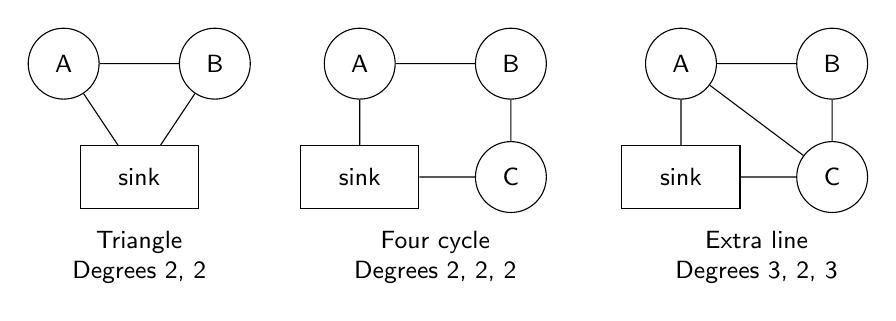
\begin{tikzpicture}[scale=.8,every node/.style={font=\small}]
\begin{scope}
\node[circle,draw,minimum size=9mm](a) at (0,1.8){A};\node[circle,draw,minimum size=9mm](b) at (2.4,1.8){B};\node[rectangle,draw,minimum width=15mm,minimum height=8mm](s) at (1.2,0){sink};
\draw(a)--(b)--(s)--(a);\node[align=center,anchor=north] at (1.2,-.7){Triangle\\Degrees 2, 2};
\end{scope}
\begin{scope}[xshift=4.7cm]
\node[circle,draw,minimum size=9mm](a) at (0,1.8){A};\node[circle,draw,minimum size=9mm](b) at (2.4,1.8){B};\node[circle,draw,minimum size=9mm](c) at (2.4,0){C};\node[rectangle,draw,minimum width=15mm,minimum height=8mm](s) at (0,0){sink};
\draw(s)--(a)--(b)--(c)--(s);\node[align=center,anchor=north] at (1.2,-.7){Four cycle\\Degrees 2, 2, 2};
\end{scope}
\begin{scope}[xshift=9.8cm]
\node[circle,draw,minimum size=9mm](a) at (0,1.8){A};\node[circle,draw,minimum size=9mm](b) at (2.4,1.8){B};\node[circle,draw,minimum size=9mm](c) at (2.4,0){C};\node[rectangle,draw,minimum width=15mm,minimum height=8mm](s) at (0,0){sink};
\draw(s)--(a)--(b)--(c)--(s);\draw(a)--(c);\node[align=center,anchor=north] at (1.2,-.7){Extra line\\Degrees 3, 2, 3};
\end{scope}
\end{tikzpicture}
\end{center}
\textbf{One legal move.} A nonsink circle needs at least one chip per line touching it. It sends exactly one chip along each line and keeps any extras. Choose one circle at a time. The sink receives chips but never shares. A stable circle has fewer chips than its degree, so it can still hold chips.

\textbf{Keep these distinctions visible}
\begin{itemize}
\item Restarting changes the experiment: restore the same initial piles and empty the sink. Merely changing move order leaves the start fixed.
\item Final piles and share counts are different data. Record one chronological firing word and the final piles. Count its A, B and C letters only after stopping; no concurrent tally is needed.
\item On the extra-line board, A and C need 3 chips. B still needs 2. Do not carry the old threshold to the new graph.
\item Chips in the sink count toward conservation, but are unavailable for later moves. No borrowing, negative chips, or moving a chip back from the sink.
\end{itemize}
\textbf{A fully worked launch trial}
\[
(2,2)\xrightarrow{A}(0,3)\xrightarrow{B}(1,1),
\qquad
(2,2)\xrightarrow{B}(3,0)\xrightarrow{A}(1,1).
\]
Both have share counts $(1,1)$ and two chips in the sink. A child may verify each arrow with counters. This is evidence for the conjecture; the general proof appears on page~\pageref{theorem}.

\textbf{Choosing hints.} First check the rules with a physical move. Then ask for a new example or a way of keeping track. Supply an organizing idea only after the child has had a real attempt. Stop an adult explanation if children want to keep experimenting. The source pedagogy in \emph{Math Circle by the Bay}, Preface pp. vii--ix, emphasizes student interaction, manipulatives, prepared fallback hints, and returning to explanations. The short launch and menu here are local design choices.

\textbf{When to stop.} A useful endpoint is a reliable pair of trials, a complete small collection, a detected addition cycle, or one convincing argument. A child need not encounter all three boards in one hour.

\newpage
\pagehead{K--1 solutions for Problems 1 to 3}
\prob{Problem 1}{Triangle starts. Changing legal move order cannot change the finish. The answer rows are:}
\begin{center}\begin{tabular}{llll}\toprule Start & Finish & Shares at each circle & One legal order\\\midrule
$(2,2)$ & $(1,1)$ & $(1,1)$ & AB\\
$(3,2)$ & $(1,0)$ & $(2,2)$ & ABAB\\
$(2,3)$ & $(0,1)$ & $(2,2)$ & ABBA\\
$(3,3)$ & $(1,1)$ & $(2,2)$ & ABAB\\
\bottomrule\end{tabular}\end{center}

The share-count column is adult support; children are only asked about final piles. These trials deliberately give three different finishes across different starts.
\hint{If a child moves just one chip, touch both lines from the firing circle and send a chip along each. For an order comparison, restore the identical start first.}
\notice{``The start matters; the order did not in our trials.'' Do not ask young children to recite a general theorem.}
\prob{Problem 2}{Distribute 4 chips altogether, then 5 altogether. Each total has exactly three possible finishes: $(1,0),(0,1),(1,1)$. The following is a complete check, with A increasing by one.}
\begin{center}\begin{tabular}{cc|cc}\toprule
4 chip start & Finish & 5 chip start & Finish\\\midrule
$(0,4)$&$(0,1)$&$(0,5)$&$(1,0)$\\
$(1,3)$&$(1,0)$&$(1,4)$&$(1,1)$\\
$(2,2)$&$(1,1)$&$(2,3)$&$(0,1)$\\
$(3,1)$&$(0,1)$&$(3,2)$&$(1,0)$\\
$(4,0)$&$(1,0)$&$(4,1)$&$(1,1)$\\
&&$(5,0)$&$(0,1)$\\\bottomrule\end{tabular}\end{center}
\textbf{Completeness.} A can hold 0 through the total; B must hold the rest. This lists every start, including empty circles. All legal orders from any listed start share its finish. With four or five chips, $(0,0)$ never occurs.
\hint{Keep the same four counters and move one from B to A between trials. Let the child decide how to keep the different finishes.}
\prob{Problem 3}{Four-cycle starts. All legal orders from a fixed start agree:}
\begin{center}\begin{tabular}{llll}\toprule Start & Finish & Shares at each circle & One legal order\\\midrule
$(0,4,0)$ & $(1,0,1)$ & $(1,3,1)$ & BBACB\\
$(2,2,0)$ & $(1,1,1)$ & $(1,1,0)$ & AB\\
$(0,2,2)$ & $(1,1,1)$ & $(0,1,1)$ & BC\\
$(2,0,2)$ & $(1,0,1)$ & $(1,1,1)$ & ACB\\
\bottomrule\end{tabular}\end{center}

\hint{B sends to A and C, not to the sink. On $(0,4,0)$, B may share twice before either neighbor shares. Ask where every chip went if the total appears to change.}

\newpage
\pagehead{K--1 solutions for Problems 4 to 6}\label{kcycle}
\prob{Problem 4}{Every stable four-cycle state has 0 or 1 chip at each circle. The complete set of eight is}
\[
(0,0,0),\ (0,0,1),\ (0,1,0),\ (0,1,1),
\qquad
(1,0,0),\ (1,0,1),\ (1,1,0),\ (1,1,1).
\]
There cannot be a stable placement of four chips: three circles hold at most one each. This is a capacity proof, not merely a failed search.
\hint{Ask how many chips one circle can hold without sharing. Once the child has examples, sort them by whether A is empty; each half has the four B/C choices.}
\notice{Changing chip positions without making moves is allowed here: this problem asks for stable placements, not outcomes from a specified start.}
\prob{Problem 5}{For every timing of additions and legal sharing, $(3,3)$ finishes at $(1,1)$, and $(2,4)$ finishes at $(1,0)$. All three repeated rows for each total have the same answer. In a batch of 3 at A then 3 at B: $(3,0)\to(1,1)$, then $(1,4)\to(1,1)$. Reversing the batch order agrees. For 2 at A then 4 at B: $(2,0)\to(0,1)$, then $(0,5)\to(1,0)$. Reversing gives $(0,4)\to(0,1)$, then $(2,1)\to(1,0)$.}
\hint{Reserve the not-yet-added chips off the board, away from the sink. Stop only after all scheduled chips have been added and no circle can share.}
\prob{Problem 6}{After adding 1 through 11 chips at A, the finishes are}
\[
(1,0),(0,1),(1,1),(1,0),(0,1),(1,1),
(1,0),(0,1),(1,1),(1,0),(0,1).
\]
No later stable finish is empty. The entire update rule on the four stable states is pictured below, so the repeating claim is exhaustive, rather than inferred only from eleven trials.
\begin{center}
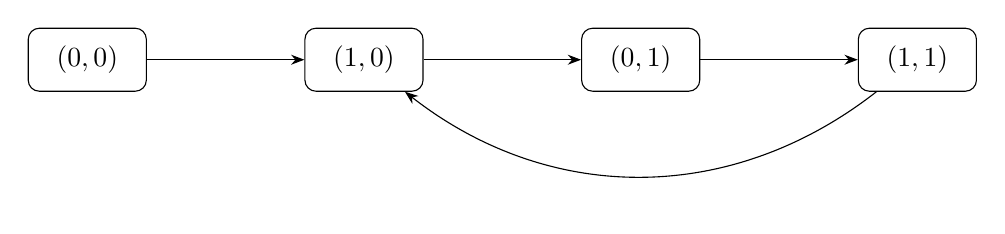
\begin{tikzpicture}[>=Stealth,every node/.style={draw,rounded corners,minimum width=15mm,minimum height=8mm},node distance=20mm]
\node (z) {$(0,0)$};\node[right=of z](a){$(1,0)$};\node[right=of a](b){$(0,1)$};\node[right=of b](c){$(1,1)$};
\draw[->](z)--(a);\draw[->](a)--(b);\draw[->](b)--(c);\draw[->](c) to[bend left=38] (a);
\end{tikzpicture}
\end{center}
Every arrow means add one at A and finish all sharing. Only the three states in the cycle occur after an addition. The initial empty state is outside the cycle.
\hint{Ask whether an arrangement has appeared before. Once it has, ask what the same next action must do from that same arrangement.}
\textbf{Concrete extension.} Repeat with additions at B and compare the same three states in the reverse cyclic order. This anticipates middle P6; use it only if the child wants another rule.

\newpage
\pagehead{Grades 2--3 solutions for Problems 1 to 3}
\prob{Problem 1}{Triangle finishes and sharing counts are both independent of legal order, for the same start.}
\begin{center}\begin{tabular}{llll}\toprule Start & Finish & Shares at each circle & One legal order\\\midrule
$(2,2)$ & $(1,1)$ & $(1,1)$ & AB\\
$(4,0)$ & $(1,0)$ & $(2,1)$ & AAB\\
$(3,3)$ & $(1,1)$ & $(2,2)$ & ABAB\\
\bottomrule\end{tabular}\end{center}

Two examples of orders are AB and BA for $(2,2)$, and ABAB and BABA for $(3,3)$. The start $(4,0)$ has only one complete legal word, AAB; the printed ``if possible'' matters. A cannot skip a legal forced move by inventing a second order.
\hint{One child moves chips and another records the firing word; then exchange roles. After stopping, count its letters to recover the sharing counts. A count at A means the number of times A shared, not chips remaining at A.}
\prob{Problem 2}{Four-cycle starts have these exact records:}
\begin{center}\begin{tabular}{llll}\toprule Start & Finish & Shares at each circle & One legal order\\\midrule
$(0,4,0)$ & $(1,0,1)$ & $(1,3,1)$ & BBACB\\
$(2,1,2)$ & $(1,1,1)$ & $(1,1,1)$ & ABC\\
$(2,4,2)$ & $(1,0,1)$ & $(3,5,3)$ & ABBABCCBACB\\
\bottomrule\end{tabular}\end{center}

Other complete words are BBCAB, CBA, and CBBCBAABCAB, respectively. Every row duplicated on the student page should end with the same finish and count vector.
\hint{If records disagree, replay the two words slowly. Check for an illegal early firing or a missed chip along the B--C edge before discussing a counterexample.}
\prob{Problem 3}{Exactly three starts of total six finish at $(1,1)$: $(0,6),(3,3),(6,0)$.}
\begin{center}\begin{tabular}{cccccccc}\toprule
A initially&0&1&2&3&4&5&6\\
B initially&6&5&4&3&2&1&0\\\midrule
Finish&$(1,1)$&$(0,1)$&$(1,0)$&$(1,1)$&$(0,1)$&$(1,0)$&$(1,1)$\\\bottomrule\end{tabular}\end{center}
\textbf{Why complete.} There are seven possible values of A, 0 through 6. Once A is chosen, B is forced. Checking these seven starts leaves none untested. Order independence means no unsuccessful start can be rescued by a new firing order.
\hint{If the child finds $(3,3)$ and stops, ask whether an empty circle is permitted at the start. If the list is disorganized, ask how one could be certain it includes every possible A pile.}
\textbf{Optional invariant for a ready child.} On the triangle, the remainder of $A-B$ upon division by 3 never changes: an A move changes it by $-3$, a B move by $+3$. The three nonempty stable pairs have different remainders. This explains the repeating pattern here. It is an extension, not a prerequisite or a replacement for the child's complete list.

\newpage
\pagehead{Grades 2--3 solutions for Problems 4 to 6}\label{middleextra}
\prob{Problem 4}{On the extra-line board, A and C have degree 3, while B has degree 2. The complete answer rows are:}
\begin{center}\begin{tabular}{llll}\toprule Start & Finish & Shares at each circle & One legal order\\\midrule
$(3,0,3)$ & $(2,0,2)$ & $(1,1,1)$ & ACB\\
$(0,6,0)$ & $(2,0,2)$ & $(1,4,1)$ & BBBACB\\
$(2,2,2)$ & $(2,0,2)$ & $(1,2,1)$ & BACB\\
$(4,1,2)$ & $(2,1,0)$ & $(2,2,2)$ & ABCABC\\
\bottomrule\end{tabular}\end{center}

Alternative legal orders, in the same row order, are CAB, BBBCAB, BCAB, and ACBABC. The added line changes thresholds and some finishes, but not the order-independence conclusion.
\hint{Before the first trial, let the child point to every destination for A's three outgoing chips. If they fire A at two chips, ask for a chip to match its third line.}
\prob{Problem 5}{The batches are 2 at A and 4 at B on the four cycle. All three timing choices finish at $(1,1,1)$. Together, $(2,4,0)$ has total firing counts $(2,3,1)$. For A's batch first, $(2,0,0)\to(0,1,0)$, then $(0,5,0)\to(1,1,1)$. For B's batch first, $(0,4,0)\to(1,0,1)$, then $(3,0,1)\to(1,1,1)$.}
\hint{Have the child name what is held back at each stage. Empty the sink between independent trials, never between the two batches of one trial.}
\prob{Problem 6}{The complete twelve-row table is below. Each rule reaches exactly $(1,0),(0,1),(1,1)$ after at least one addition. $(0,0)$ occurs only before the first addition.}
\begin{center}\begin{tabular}{ccc}\toprule
Chips added & Add at A then finish & Add at B then finish\\\midrule
1&$(1,0)$&$(0,1)$\\2&$(0,1)$&$(1,0)$\\3&$(1,1)$&$(1,1)$\\
4&$(1,0)$&$(0,1)$\\5&$(0,1)$&$(1,0)$\\6&$(1,1)$&$(1,1)$\\
7&$(1,0)$&$(0,1)$\\8&$(0,1)$&$(1,0)$\\9&$(1,1)$&$(1,1)$\\
10&$(1,0)$&$(0,1)$\\11&$(0,1)$&$(1,0)$\\12&$(1,1)$&$(1,1)$\\\bottomrule\end{tabular}\end{center}
\textbf{Why the cycles persist.} The A-addition map is drawn on page~\pageref{kcycle}. Interchanging the names A and B gives the B-addition map. Once the same pair recurs, the fixed rule repeats the same successors forever. The two rules traverse the three-cycle in opposite directions.
\hint{An adult may turn a child's repeated rows into three state cards with arrows. Introduce the diagram after the repetition has a purpose.}

\newpage
\pagehead{Grades 4--5 solutions for Problems 1 to 4}
\prob{Problem 1}{For one fixed start, final piles cannot agree while share counts differ. Here are all four records:}
\begin{center}\begin{tabular}{llll}\toprule Start & Finish & Shares at each circle & Chips in sink\\\midrule
$(2,2)$ & $(1,1)$ & $(1,1)$ & 2\\
$(4,0)$ & $(1,0)$ & $(2,1)$ & 3\\
$(3,3)$ & $(1,1)$ & $(2,2)$ & 4\\
$(5,4)$ & $(1,0)$ & $(4,4)$ & 8\\
\bottomrule\end{tabular}\end{center}

Use AB/BA; AAB only; ABAB/BABA; and AABABBAB/BBAABAAB, respectively. Across \emph{different} starts, equal finishes with different share counts do occur: $(2,2)$ and $(3,3)$ are examples. Preserve the printed fixed-start qualification.
\prob{Problem 2}{Together, first batch then second, and second then first all give the same finish for each row group:}
\begin{center}\begin{tabular}{llll}\toprule
Batches & Together & First then second & Second then first\\\midrule
4 at B; 2 at A&$(1,1,1)$&$(1,1,1)$&$(1,1,1)$\\
3 at A; 3 at C&$(1,0,1)$&$(1,0,1)$&$(1,0,1)$\\\bottomrule\end{tabular}\end{center}
For the first pair, intermediate finishes are $(1,0,1)$ or $(0,1,0)$, as appropriate. For the second pair, $(3,0,0)\to(1,1,0)$, then $(1,1,3)\to(1,0,1)$; reversing A/C gives $(0,1,1)$ then $(3,1,1)\to(1,0,1)$. This does not claim the intermediate states agree.
\hint{Compare only after the same total additions have arrived and sharing is finished.}
\prob{Problem 3}{The four stable starts have the following A-addition updates:}
\begin{center}\begin{tabular}{ccccc}\toprule
Start&After 1&After 2&After 3&After 4\\\midrule
$(0,0)$&$(1,0)$&$(0,1)$&$(1,1)$&$(1,0)$\\
$(1,0)$&$(0,1)$&$(1,1)$&$(1,0)$&$(0,1)$\\
$(0,1)$&$(1,1)$&$(1,0)$&$(0,1)$&$(1,1)$\\
$(1,1)$&$(1,0)$&$(0,1)$&$(1,1)$&$(1,0)$\\\bottomrule\end{tabular}\end{center}
The three nonempty starts return after three additions and then at multiples of three. The empty start never returns. Starts $(0,0)$ and $(1,1)$ merge after one addition at $(1,0)$: the operation cannot be reversed uniquely. The state diagram on page~\pageref{kcycle} is complete.
\hint{Ask which arrows could be reversed without making a choice. Do not label all stable states a group.}
\prob{Problem 4}{Extra-line answers: $(3,0,3)\to(2,0,2)$ with counts $(1,1,1)$; $(0,6,0)\to(2,0,2)$ with counts $(1,4,1)$; $(4,1,2)\to(2,1,0)$ with counts $(2,2,2)$. Orders from page~\pageref{middleextra} give two trials for each. Legal order still changes neither record.}

\newpage
\pagehead{Grades 4--5 solutions for Problems 5 and 6}
\prob{Problem 5}{All three 12-chip starts stop. They happen to share one finish, although their share counts differ:}
\begin{center}\begin{tabular}{llll}\toprule Start & Finish & Shares at each circle & Chips in sink\\\midrule
$(0,12,0)$ & $(1,0,1)$ & $(5,11,5)$ & 10\\
$(6,0,6)$ & $(1,0,1)$ & $(5,5,5)$ & 10\\
$(4,4,4)$ & $(1,0,1)$ & $(5,7,5)$ & 10\\
\bottomrule\end{tabular}\end{center}

\textbf{A finite score proves termination on this board.} Give each chip at A or C a score of 3, each at B a score of 4, and each at the sink a score of 0. The total $W=3A+4B+3C$ is a nonnegative integer. An A or C move removes two 3-point chips and creates one 4-point chip, decreasing $W$ by 2. A B move removes two 4-point chips and creates two 3-point chips, also decreasing $W$ by 2. Therefore infinitely many legal moves are impossible. This works for every finite start and every choice of legal moves on the four cycle. The three starts have scores 48, 36, 40; each finishes at score 6, so the total numbers of moves are 21, 15, 17.
\hint{First ask why ``a chip falls into the sink every move'' is false: B does not touch the sink. For a child who wants a numerical certificate, give the 3,4,3 weights and let them test each type of move.}
\prob{Problem 6}{From $(0,8,0)$, the unique finish is $(1,0,1)$, with counts $(3,7,3)$ and 6 chips in the sink. Two full legal words are BBABBABCCBACB and BBCBBCBAABCAB. Each has 13 moves. They exchange A and C choices.}
\textbf{Why the share counts must agree.} Fix one finished legal history, with $u_v$ shares at each circle $v$. Imagine another legal history, and suppose it is about to be the first to exceed one of those quotas, at $v$. So far, $v$ has shared exactly $u_v$ times, and every neighbor has shared no more than its quota. Thus $v$ has received no more chips than in the finished history and has sent exactly as many. Its present pile is at most its pile in that stable finish. It cannot legally share. This contradiction says no quota can be exceeded. If the other history also finishes, reverse the comparison; all quotas are equal. Equal counts determine equal final piles.

\textbf{Child-facing proof conversation.} Write the quotas 3,7,3 beside the sample board. Ask, ``Could a different run be the first to make A share a fourth time? Before that happens, could A have received more chips than in our finished run?'' Then discuss the same question for B and C. A careful explanation of that comparison is enough; symbolic notation is optional.
\textbf{Arithmetic check for this instance}
\[
A_{\rm end}=0-2(3)+7=1,\quad
B_{\rm end}=8-2(7)+3+3=0,\quad
C_{\rm end}=0-2(3)+7=1.
\]
The score drops from 32 to 6, hence $(32-6)/2=13$ moves. A score proves the run stops; the quota argument proves every legal completed run has the same per-circle counts.

\newpage
\pagehead{General reasoning and optional extensions}
\textbf{Termination beyond the four cycle.} On any finite connected undirected graph with a sink, an infinite legal run would make some circle fire infinitely often. Every neighbor would then receive infinitely many chips. Since the total chip supply is finite, that neighbor must also fire infinitely often. Follow a path to the sink: a neighbor of the sink would fire infinitely often, sending infinitely many chips permanently into it. That is impossible with a finite supply. No fairness assumption about choosing active circles is needed. Connectedness to the absorbing sink is essential.

\textbf{Staged additions.} Let $S(x)$ mean the stable finish from $x$. A legal history for $x$ is still legal if an extra nonnegative batch $y$ is present from the start. Running that history leaves $S(x)+y$; finishing it therefore agrees with finishing $x+y$ directly. The uniqueness argument yields
\[
S(S(x)+y)=S(x+y).
\]
The same idea works when individual additions are interleaved with legal moves: move all the prescribed additions to the beginning. Every original move stays legal. After all additions and all sharing, the final state is unchanged. This justifies K--1 P5 as well as both older batch problems.

\textbf{A small algebraic extension.} On stable states define $x\mathbin{\oplus}y=S(x+y)$. This operation is commutative and associative by the staged-addition identity. It need not be cancellative or reversible, as upper P3 demonstrates. The full four-state set on the triangle is not a group; do not infer group structure from one three-cycle.

\textbf{Further questions with known endpoints}
\begin{itemize}
\item On the extra-line board, find every stable placement. There are $3\cdot2\cdot3=18$, since A/C may hold 0,1,2 and B may hold 0,1. At most 5 chips can be stable; $(2,1,2)$ attains this.
\item On the four cycle, seek a start that finishes empty. The only such start is the empty one. A last legal move, if present, sends at least one chip to another nonsink circle, so it cannot produce the empty state. This argument also works on the other two printed graphs, but not on a graph with a lone circle attached only to a sink.
\item Remove the sink rule from the triangle and use three ordinary vertices of degree 2. Start $(2,1,0)$. Firing the first, second, third vertices successively returns to $(2,1,0)$: $(0,2,1)$ then $(1,0,2)$ then the start. Termination fails. Clearly separate this changed game from the packet rules.
\end{itemize}
\textbf{Sources and fidelity limits.} Holroyd, Levine, M\'esz\'aros, Peres, Propp, and Wilson, \emph{Chip-Firing and Rotor-Routing on Directed Graphs}, \S2, Lemmas 2.2--2.5 and Corollary 2.6, manuscript pp. 3--5: \url{https://arxiv.org/abs/0801.3306}. Levine and Propp, \emph{What is a sandpile?}, manuscript pp. 1--2 (least-action characterization on p. 2): \url{https://lionellevine.github.io/what-is-a-sandpile.pdf}. These supply finite-sink mathematics; this guide restricts to the undirected printed boards. The explicit instances, score proof, hints, menu, and check code are local adaptations, not tested lessons from those sources. Givental, Nemirovskaya, and Zakharevich, \emph{Math Circle by the Bay} (AMS, 2018), Preface pp. vii--ix, supplies the pedagogical observations noted on page~\pageref{boards}.

\textbf{Verification and use record.} Independent exhaustive branching checked every assigned numerical start, including totals 4,5,6, and all four repeated-addition starts. Every branch has one terminal state and one count vector. This is evidence for the finite instances; the arguments above cover arbitrary finite starts. Record actual attendance, problems attempted, needed hints, and children's explanations after use. Do not mark this draft piloted until that happens.

\end{document}
